The router adopts a two-way flow-control mechanism that combines a forward valid-ready handshake with backward credit return. The forward path transfers the flit data and its associated control information, while the backward path reports buffer-release events from the downstream router through \texttt{credit\_return}. Together, these mechanisms determine when a flit can safely move to the next router. This flow-control mechanism is illustrated in Fig.~\ref{fig:handshake_and_credit-based_flow_control}.

\begin{figure}[htbp]
    \centering
    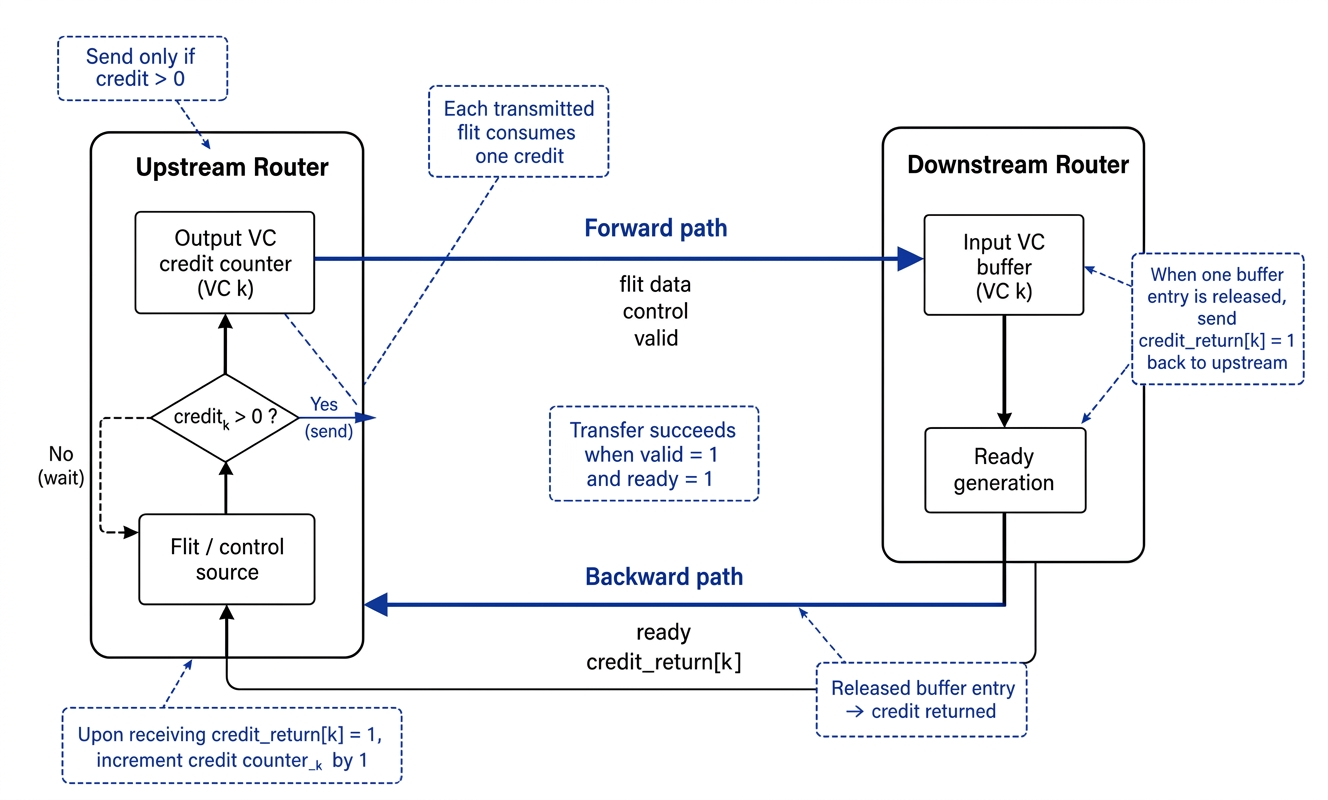
\includegraphics[width=0.85\textwidth]{images/ch3_design_and_implementation/handshake.png}
    \caption{Valid-ready handshake and credit-based flow control between neighboring routers.}
    \label{fig:handshake_and_credit-based_flow_control}
\end{figure}

In the forward path, a flit transfer is completed only when \texttt{valid} and \texttt{ready} are both asserted in the same clock cycle. The \texttt{valid} signal is generated by the sender to indicate that the current flit and its control fields are available, while \texttt{ready} is generated by the receiver to indicate that it can accept the flit in the current cycle. If \texttt{valid} is high but \texttt{ready} is low, the sender keeps the current flit and control signals stable until the handshake succeeds.

The credit return path is used to track the availability of downstream virtual-channel buffers. When \texttt{credit\_return[k] = 1}, one buffer entry in downstream input virtual channel \texttt{k} has been released. The upstream router then increments the corresponding output virtual-channel credit counter. Before scheduling a flit to an output virtual channel, the router checks whether the corresponding credit count is non-zero. A flit can be selected for transmission only when downstream buffer space is available, and each successful advancement consumes one credit.

In this design, the valid-ready handshake controls whether a flit is transferred in the current cycle, while the credit mechanism tracks downstream buffer availability across cycles. By combining these two mechanisms, the router avoids downstream buffer overflow and propagates backpressure when congestion occurs. This provides controlled and reliable flow-control behavior for pipelined flit transmission.
